\documentclass[12pt]{article}
\usepackage[utf8]{inputenc}
\usepackage{amsmath}
\usepackage{amsfonts}
\usepackage{amssymb}
\usepackage{empheq}
\usepackage{graphicx}
\usepackage{tikz}
\usepackage{changepage}
\usetikzlibrary{automata, positioning, arrows, shapes}
\addtolength{\topmargin}{-0.875in}
\addtolength{\textheight}{1.75in}
\title{Math 332 A - Mathematical Statistics}
\author{Ethan Jensen}
\date{April 3, 2020}

\begin{document}
	\maketitle HW p.378 \#48,52,54,\ \ p.379 \#58,66
	\section[20pt]{p. 378 \#48}
	In a random sample, the weights of 24 Black Angus steers of a certain age have a standard deviation of 238 pounds. Assuming that the weights constitue a random sample from a normal population, test the null hypothesis \(\sigma = 250\) pounds against the two sided alternative \(\sigma = 250\) pounds at the 0.01 level of significance.
	\newline \newline
	We have
	\newline
	\(H_0: \sigma = 250\)
	\newline
	\(H_1: \sigma \neq 250\)
	\newline
	\(\alpha = 0.01\)
	\newline \newline
	From \(H_1\), we must use a two-tailed test. To be accepted, the following must be true:
	\[\chi^2_{1-\alpha/2, n-1} \leq \frac{(n-1)s^2}{\sigma^2} \leq \chi^2_{\alpha/2, n-1}\]
	Plugging in \(n=24, \alpha = 0.01, s = 238\) and using Table V we have
	\[9.260 \leq \frac{23}{\sigma^2}(238)^2\leq 44.181\]
	\[0.40261 \leq \frac{(238)^2}{\sigma^2} \leq 1.92091\]
	\[0.63451 \leq \frac{238}{\sigma} \leq 1.38597\]
	\[0.72152 \leq \frac{\sigma}{238} \leq 1.57602\]
	\[171.7218 \leq \sigma \leq 375.0926\]
	\(\sigma = 250\) falls into the acceptance region.
	\newline
	\boxed{\textup{We accept the null hypothesis, }\sigma = 250}
	\newpage
	\section[20pt]{p. 378 \#52}
	With reference to Exercise 13.51, find the P-value corresponding with the observed value of the test statistic and use it to decide whether the null hypothesis could have been rejected at the 0.015 level of significane.
	\newline \newline
	With reference to Exercise 13.51, we have
	\newline
	\(H_0: \sigma = 0.41\)
	\newline
	\(H_1: \sigma > 0.41\)
	\newline
	\(\alpha = 0.015\)
	\newline
	\(n = 50, s = 0.49\)
	\newline \newline
	From \(H_1\), we must use a one-tailed test. To be accepted, the following must be true:
	\[\frac{(n-1)s^2}{\sigma^2} \leq \chi^2_{\alpha, n-1}\]
	Plugging in \(n=50, s = 0.49, \sigma = 0.41\)
	\[\frac{49\cdot 0.49^2}{0.41^2} \leq \chi^2_{\alpha, n-1}\]
	\[\chi^2_{\alpha, n-1} \geq 69.9875\]
	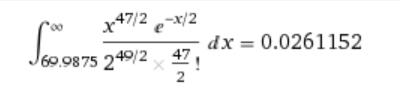
\includegraphics{spicy integral 3}
	\newline
	So we have a P-value of 0.0261152.
	\newline \newline
	\boxed{\textup{Since }\alpha = 0.015 \textup{ is less than our P-value, we accept the null hypothesis.}}
	\newpage
	\section[20pt]{p. 378 \#54}
	With reference to Exercise 13.40, test at the 0.10 level of significance whether it is reasonable to assume that the two populations sampled have equal variances.
	\newline \newline
	From Exercise 13.40, we know that \(s_1 = 3.3, s_2 = 2.1, n_1 = 6, n_2 = 6\) and that the populations sampled are normal.
	\newline \newline
	\(H_0:\ \sigma^2_1 = \sigma^2_2\)
	\newline
	\(H_1:\ \sigma^2_1 \neq \sigma^2_2\)
	\newline
	\(\alpha = 0.10\)
	\newline \newline
	Using an online table,
	\[f_{0.10, 6,6} = 3.05455\]
	\[\frac{s_1^2}{s_2^2} = \frac{3.3^2}{2.1^2} = 2.25\]
	This is less than \(f_{0.10, 6,6} = 3.05455\).
	\newline
	\boxed{\textup{It is reasonable to assume the variances are equal.}}
	\newpage
	\section[20pt]{p. 379 \#58}
	With reference to Exercise 13.57, find the critical region and the actual level of significance corresponding to this critical region.
	\newline \newline
	\(H_0: \theta = 0.40\)
	\newline
	\(H_1: \theta > 0.40\)
	\newline \newline
	The critical region is the region corresponding to a rejection of the null hypothesis. We want to maximize this region without rejecting the null hypothesis given our data.
	\newline
	Thus, the following equation must hold.
	\[\sum_{k=10}^{18}\binom{18}{k}\theta^k(1-\theta)^{18-k} \geq \alpha\]
	where \(\alpha\) is the level of significance corresponding to this region.
	\newline \newline
	The back of the book says that this sum is equal to 0.1348.
	\newline
	\boxed{\textup{The critical region is }\{11,12,...18\} \textup{ with a significance of } 0.1348}
	\newpage
	\section[20pt]{p. 379 \#66}
	In a random sample of 600 cars making a right turn at a certain intersection, 157 pulled into the wrong lane. Use the 0.05 level of significance to test the null hypothesis that the actual proportion of drivers who make this mistake at the given intersection is \(\theta = 0.30\) against the alternative hypothesis \(\theta \neq 0.30\).
	\newline \newline
	\(H_0:\ \theta = 0.30\)
	\newline
	\(H_1:\ \theta \neq 0.30\)
	\newline
	\(\alpha = 0.05\)
	\newline \newline
	Since n is really big, we can use a normal approximation for the binomial random variable representing the number of drivers who make the mistake.
	\newline
	\[z = \frac{x-n\theta}{\sqrt{n\theta(1-\theta)}}\]
	is approximately a standard normal distribution.
	\newline
	Since z is symmetric, a maximal critical region is symmetric.
	\newline
	So we want \(|z| \leq z_{\alpha/2}\).
	\newline
	\[z = \frac{157-180}{\sqrt{180(0.7)}} = \frac{23}{\sqrt{126}} = -2.049\]
	\[|z| = 2.049\]
	\[z_{\alpha/2} = z_{0.025} = 2.807\]
	\boxed{\textup{Since }|z| \leq z_{\alpha/2}\textup{, we accept the null hypothesis.}}
\end{document}
